\documentclass{article}

\usepackage{hyperref}
\hypersetup{
    colorlinks,
    citecolor=black,
    filecolor=black,
    linkcolor=black,
    urlcolor=black
}

\renewcommand*\descriptionlabel[1]{\hspace\leftmargin$#1$}

\usepackage[a4paper, margin=3cm]{geometry}
\usepackage{parskip}

\usepackage{amssymb}
\usepackage{amsmath}
\usepackage[ruled, vlined]{algorithm2e}
\usepackage{inconsolata}

\usepackage{graphicx}

\usepackage{subfig}
\everymath{\mathtt{\xdef\tmp{\fam\the\fam\relax}\aftergroup\tmp}}
\everydisplay{\mathtt{\xdef\tmp{\fam\the\fam\relax}\aftergroup\tmp}}

\begin{titlepage}
    \title{2802ICT Intelligent Systems Assignment 2}
    \author{Michael Ellicott \\ s5276830}
    \date{\today}
\end{titlepage}

\begin{document}



\maketitle
\newpage


\tableofcontents
\newpage

\section{Classification using Decision Trees}

\subsection{Software Design}

\begin{list}{-}{}
    \item Node class
    \item DecisionTree class
\end{list}


\subsection{Experiments}

\subsection{Findings}

\newpage

\section{Neural Networks}

\subsection{Software Design}

\begin{list}{-}{}
    \item NeuralNetwork class
    \item structure
\end{list}


\subsection{Experiments}

\begin{figure}[!ht]
    \begin{tabular}{cc}
    \subfloat{\includegraphics[width=\textwidth]{"Figure_1.png"}} &
    \end{tabular}
    \caption{Comparison}
\end{figure}

\begin{figure}
    \centering
    \begin{tabular}{cc}
    \subfloat[mbs = 1,   lr = 0.1]{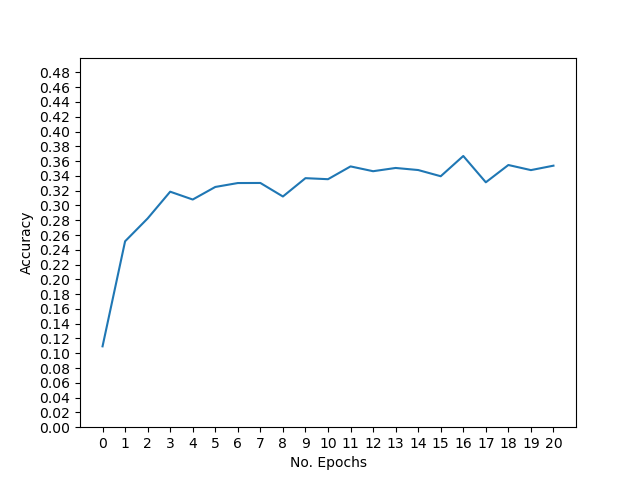
\includegraphics[width=0.5\textwidth]{"figures/fig_0.png"}} &
    \subfloat[mbs = 5,   lr = 0.1]{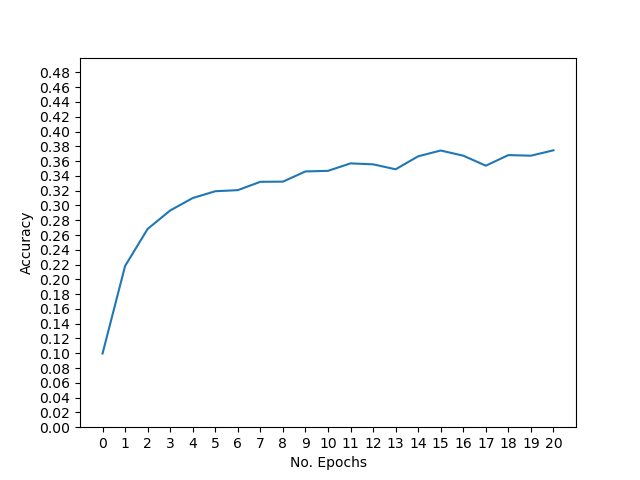
\includegraphics[width=0.5\textwidth]{"figures/fig_1.png"}} \\
    \subfloat[mbs = 20,  lr = 0.1]{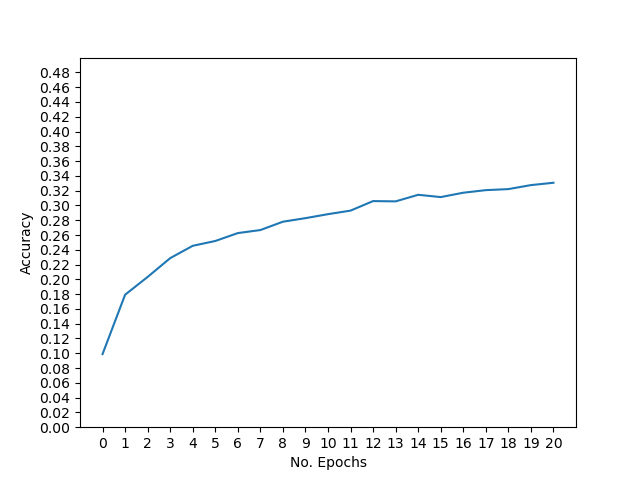
\includegraphics[width=0.5\textwidth]{"figures/fig_2.png"}} &
    \subfloat[mbs = 300, lr = 0.1]{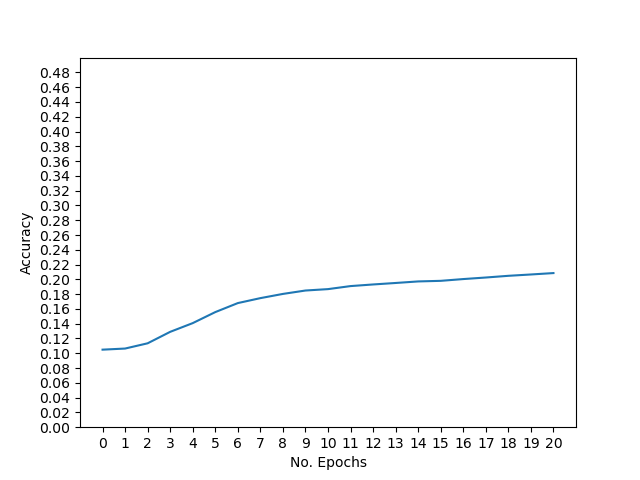
\includegraphics[width=0.5\textwidth]{"figures/fig_3.png"}} \\
    \end{tabular}
    \caption{Effect of mini-batch size on accuracy over epochs}
\end{figure}

\begin{figure}
    \centering
    \begin{tabular}{cc}
    \subfloat[mbs = 100, lr = 0.001]{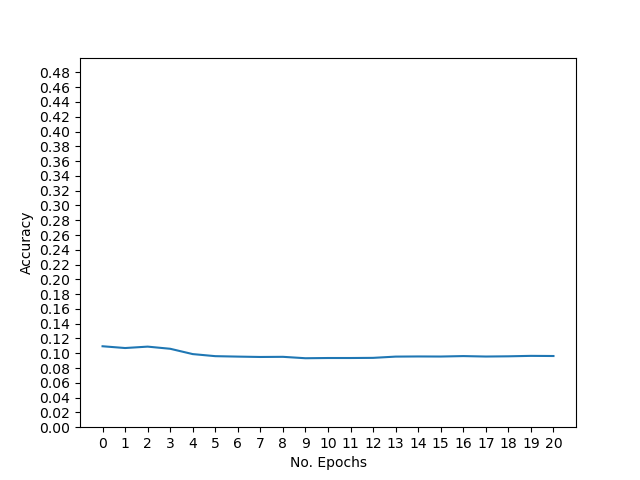
\includegraphics[width=0.5\textwidth]{"figures/fig_4.png"}} &
    \subfloat[mbs = 100, lr = 0.01 ]{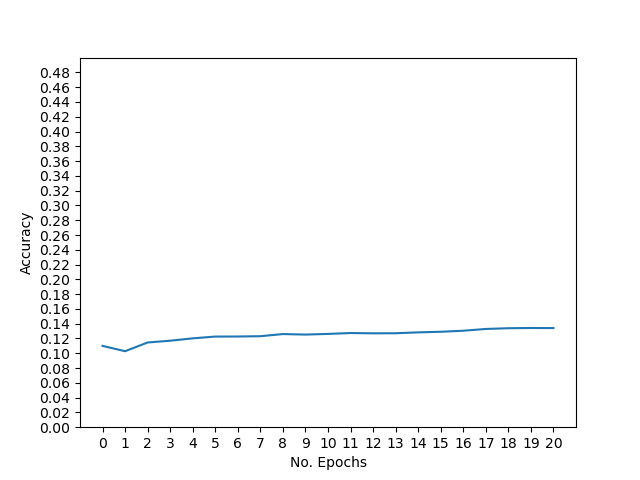
\includegraphics[width=0.5\textwidth]{"figures/fig_5.png"}} \\
    \subfloat[mbs = 100, lr = 0.1  ]{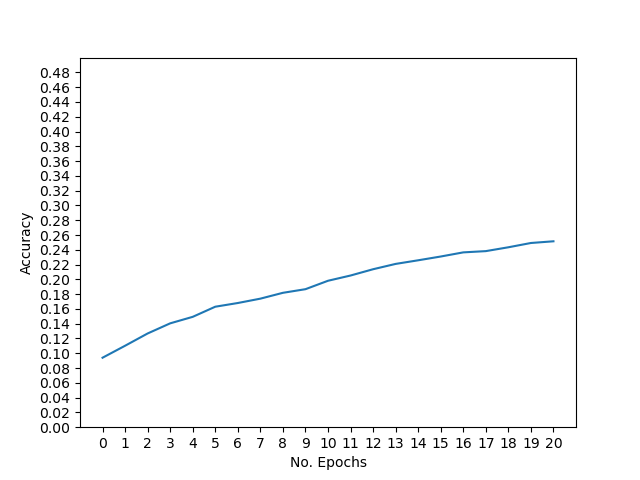
\includegraphics[width=0.5\textwidth]{"figures/fig_6.png"}} &
    \subfloat[mbs = 100, lr = 1.0  ]{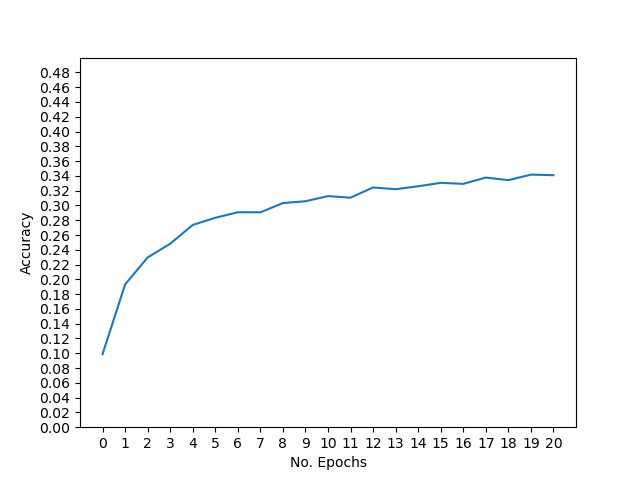
\includegraphics[width=0.5\textwidth]{"figures/fig_7.png"}} \\
    \subfloat[mbs = 100, lr = 10   ]{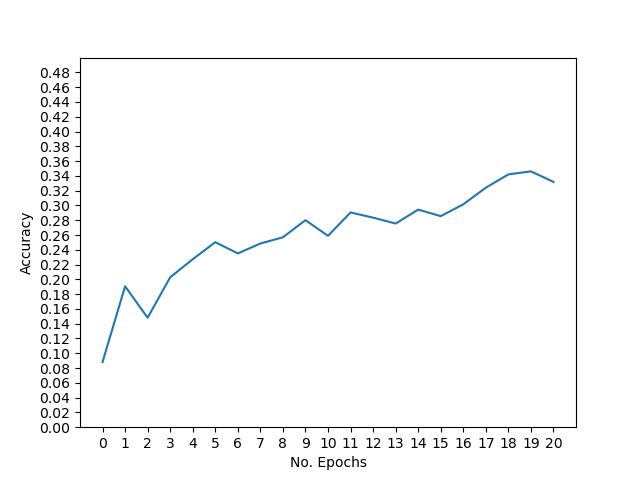
\includegraphics[width=0.5\textwidth]{"figures/fig_8.png"}} &
    \end{tabular}
    \caption{Effect of learning rate on accuracy over epochs}
\end{figure}


\newpage

\subsection{Findings}
Some text belongs here.


\section*{Conclusion}
Neural networks are good.


\newpage



\section*{Conclusion}

Classification is one example of machine learning.

\paragraph{Decision Trees}
Decision trees are useful for BLAH BLAH BLAH but they are limited in the
kind of input they can accept. They are unable to identify visual
patterns, so they cannot be used for image classification.

\paragraph{Neural Networks}
Neural networds are useful for more complex classifcation problems.

Mini-batch size and learning rate both have a significant impact on
the performance of a neural network. Too low of a mini-batch size and
(EFFECT OF MBS). Too low of a learning rate drastically increases the
amount of training time required, while too high of a learning rate
tends to get the model stuck in a local optima.

When using a 3-layer neural network (3072 - 30 - 10) to classify images from
the cifar-10 dataset, a mini-batch size of 5 and a learning rate of 1
appear to provide the greatest error reduction in the least amount of
time.




\end{document}